%%%%%%%%%%%%%%%%%%%%%%%%%%%%%%%%%%%%%%%%%
% University/School Laboratory Report
% LaTeX Template
% Version 3.1 (25/3/14)
%
% This template has been downloaded from:
% http://www.LaTeXTemplates.com
%
% Original author:
% Linux and Unix Users Group at Virginia Tech Wiki 
% (https://vtluug.org/wiki/Example_LaTeX_chem_lab_report)
%
% License:
% CC BY-NC-SA 3.0 (http://creativecommons.org/licenses/by-nc-sa/3.0/)
%
%%%%%%%%%%%%%%%%%%%%%%%%%%%%%%%%%%%%%%%%%

%----------------------------------------------------------------------------------------
%	PACKAGES AND DOCUMENT CONFIGURATIONS
%----------------------------------------------------------------------------------------

\documentclass{article}

\usepackage[version=3]{mhchem} % Package for chemical equation typesetting
\usepackage{siunitx} % Provides the \SI{}{} and \si{} command for typesetting SI units
\usepackage{graphicx} % Required for the inclusion of images
\usepackage{natbib} % Required to change bibliography style to APA
\usepackage{amsmath} % Required for some math elements 
\usepackage{enumitem}

\setlength\parindent{0pt} % Removes all indentation from paragraphs

\renewcommand{\labelenumi}{\alph{enumi}.} % Make numbering in the enumerate environment by letter rather than number (e.g. section 6)

%\usepackage{times} % Uncomment to use the Times New Roman font

%----------------------------------------------------------------------------------------
%	DOCUMENT INFORMATION
%----------------------------------------------------------------------------------------

\title{Tutorial 1\\ X Ray Diffraction \\ } % Title

\author{Linda \textsc{Crandall} and Maggie \textsc{Huff}} % Author name

\date{\today} % Date for the report

\begin{document}

\maketitle % Insert the title, author and date

\begin{center}
\begin{tabular}{l r}
Date Performed: & June 7, 2017 \\ % Date the experiment was performed
Instructor: & Chris Pratt % Instructor/supervisor
\end{tabular}
\end{center}

% If you wish to include an abstract, uncomment the lines below
% \begin{abstract}
% Abstract text
% \end{abstract}

%----------------------------------------------------------------------------------------
%	SECTION 1
%----------------------------------------------------------------------------------------

\section{Objective}

To get to know the diffractometer and X'Pert Data Collector 
%(as defined in \ref{definitions}):

%\begin{center}\ce{2 Mg + O2 -> 2 MgO}\end{center}

% If you have more than one objective, uncomment the below:
%\begin{description}
%\item[First Objective] \hfill \\
%Objective 1 text
%\item[Second Objective] \hfill \\
%Objective 2 text
%\end{description}


\section{Results and Conclusions}

Scan 4 is the best to use for {422} planes in Silicon; it uses a time per step of .5 seconds over a 1 degree range and .02 degrees step size. The large and small peaks of $CuK_\alpha1$ and $CuK_\alpha2$ do appear to be very close to a 2:1 ratio in intensity. 

\begin{figure}[h]
\begin{center}
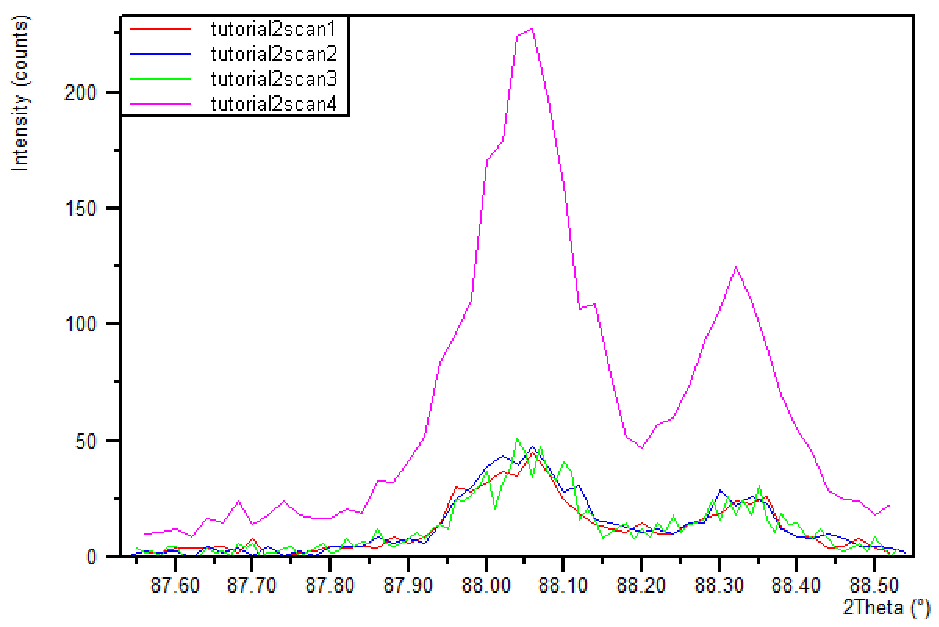
\includegraphics[width=0.65\textwidth]{combinedgraph} % Include the image combinedgraph.pdf
\caption{{422} plane in Si sample with Cu target: K$\alpha_1$ and K$\alpha_2$ peaks, variable step size, scan time, time per step}
\end{center}
\end{figure}

%----------------------------------------------------------------------------------------
%	SECTION 5
%----------------------------------------------------------------------------------------

\section{Discussion}
Increasing the scan time lets in more signal, but also lets in more background. Increasing the step size makes the peaks less noisy. Using continuous scan mode instead of step mode makes the scan time shorter. 


%----------------------------------------------------------------------------------------
%	SECTION 6
%----------------------------------------------------------------------------------------

\section{Answers to Multiple Choice Questions}
\begin{enumerate}[label=(\roman*)]
\begin{item}
d
\end{item}
\begin{item}
c
\end{item}
\begin{item}
c
\end{item}
\begin{item}
b
\end{item}

\end{enumerate}

%----------------------------------------------------------------------------------------
%	BIBLIOGRAPHY
%----------------------------------------------------------------------------------------

\bibliographystyle{apalike}

\bibliography{sample}

%----------------------------------------------------------------------------------------


\end{document}